%\addtorecentlist{secnumdepth}

\begin{saveblock}{standalone}
    \begin{highlightblock}[linewidth=\textwidth,gobble=8]
        % Bestand: prachtigeformule.tex
        \documentclass{standalone}
        \usepackage{amsmath,amssymb}

        \begin{document}
            $\displaystyle\sum_{k=0}^{\infty}
            \frac{x^k}{k!}=e^{x}$
        \end{document}
    \end{highlightblock}
\end{saveblock}

\begin{frame}
    \frametitle{Standalone}

    \centering

    \useblock{standalone}

    \hll|\\includegraphics[...]\{prachtigeformule.pdf\}|

    \medskip
    \adjustbox{cfbox=black 1pt 0pt}{%
    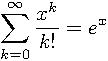
\includegraphics[width=\linewidth,height=40pt,keepaspectratio]{assets/document-standalone.pdf}%
    }
    
    % \begin{columns}
    %     \begin{column}{0.5\textwidth}
    %         \useblock{standalone}
    %     \end{column}
    %     \begin{column}{0.5\textwidth}
    %         \hll|\\includegraphics[...]\{standalone.pdf\}|

    %         \medskip
    %         \adjustbox{cfbox=black 1pt 0pt}{%
    %         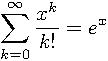
\includegraphics[width=\linewidth,height=0.8\textheight,keepaspectratio]{assets/document-standalone.pdf}%
    %         }
    %     \end{column}
    % \end{columns}
\end{frame}

\definecolor{imagebackground}{RGB}{247,247,247}


\begin{frame}
    \frametitle{Raster vs vector graphics}

    \begin{columns}
        \begin{column}{0.5\textwidth}
            \centering
            \textbf{Raster} (.png, .jpg, .jpeg, .bmp)
            \medskip

            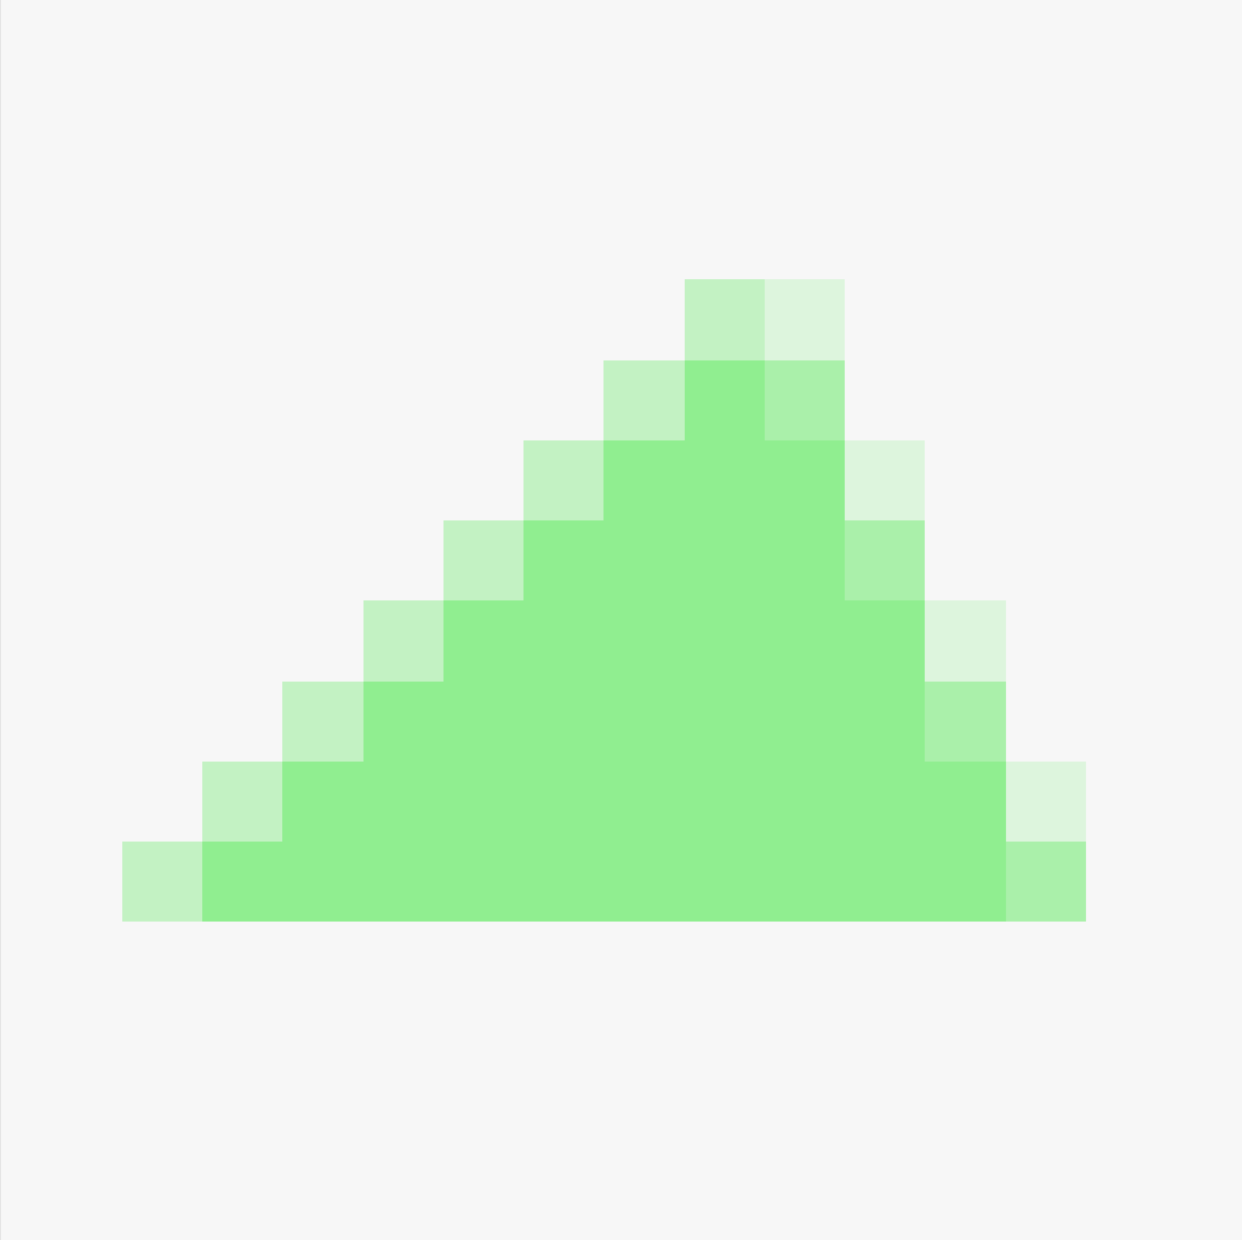
\includegraphics[width=0.8\textwidth]{assets/vector_vs_raster-vector-rasterized2_scaled.png}
        \end{column}
        \begin{column}{0.5\textwidth}
            \centering 
            \textbf{Vector} (.pdf, .svg, .dvi, .ps)
            \medskip

            \adjustbox{bgcolor=imagebackground}{%
            
\includegraphics[width=0.8\textwidth]{assets/vector_vs_raster-vector.pdf}%
            }
        \end{column}
    \end{columns}
\end{frame}

\begin{frame}
    \frametitle{Raster vs vector graphics}

    \centering

    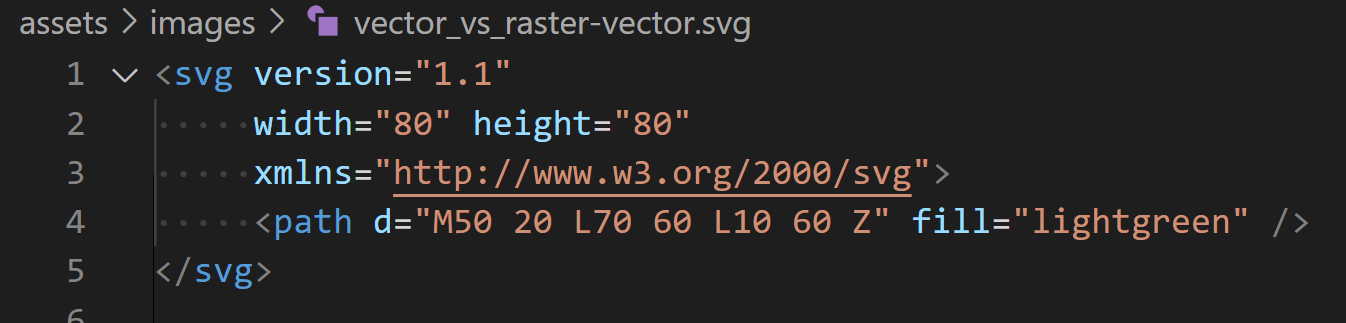
\includegraphics[width=\textwidth]{assets/vector_vs_raster-vector_code.png}

    \adjustbox{fbox=1pt 0pt}{%
        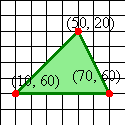
\includegraphics[height=0.4\textheight]{assets/vector_vs_raster-vector-annotated_grid.pdf}%
    }\quad
    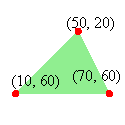
\includegraphics[height=0.4\textheight]{assets/vector_vs_raster-vector-annotated.pdf}%
    \quad
    
\includegraphics[height=0.4\textheight]{assets/vector_vs_raster-vector.pdf}

\end{frame}

\begin{frame}
    \centering

    \begin{onlyenv}<+>
        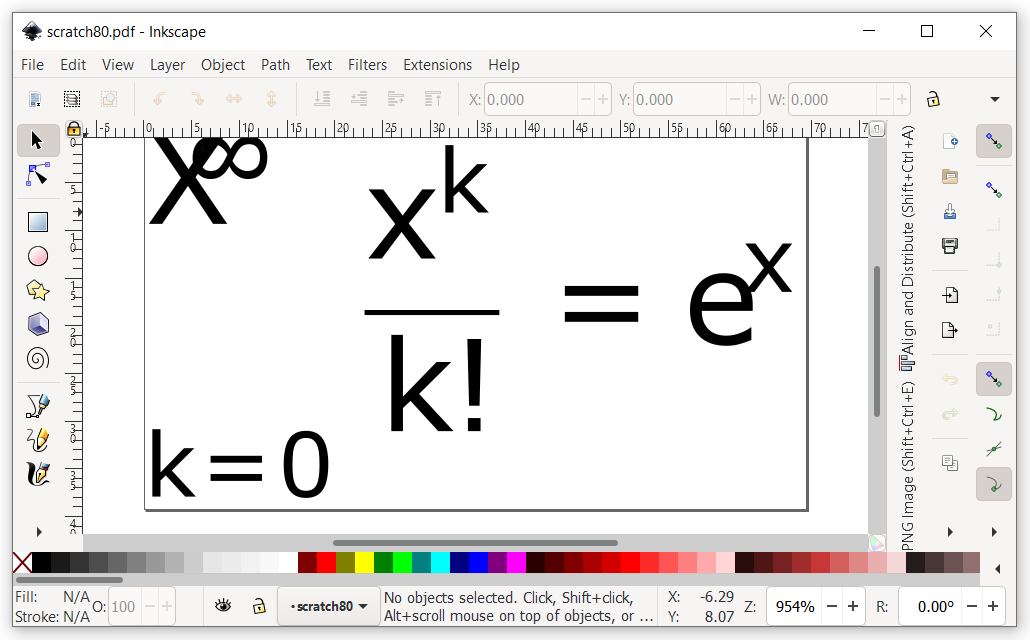
\includegraphics[width=\textwidth,height=0.8\textheight,keepaspectratio]{assets/document-loadinscape-aspdf.png}
    \end{onlyenv}
    \begin{onlyenv}<+>
        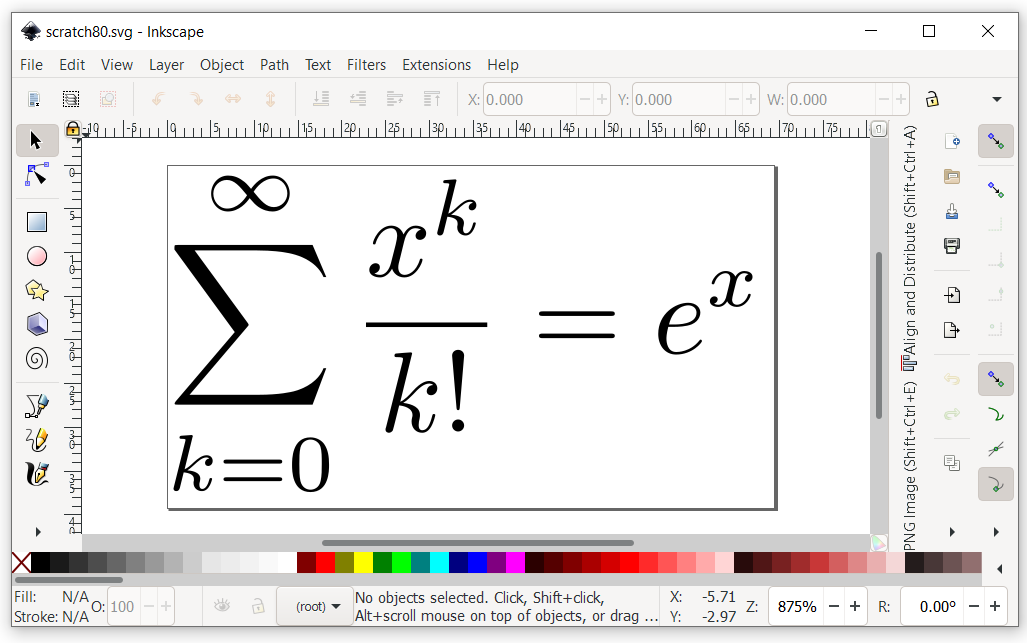
\includegraphics[width=\textwidth,height=0.8\textheight,keepaspectratio]{assets/document-loadinscape-assvg.png}
    \end{onlyenv}
\end{frame}

\begin{frame}
    \begin{onlyenv}<+>
        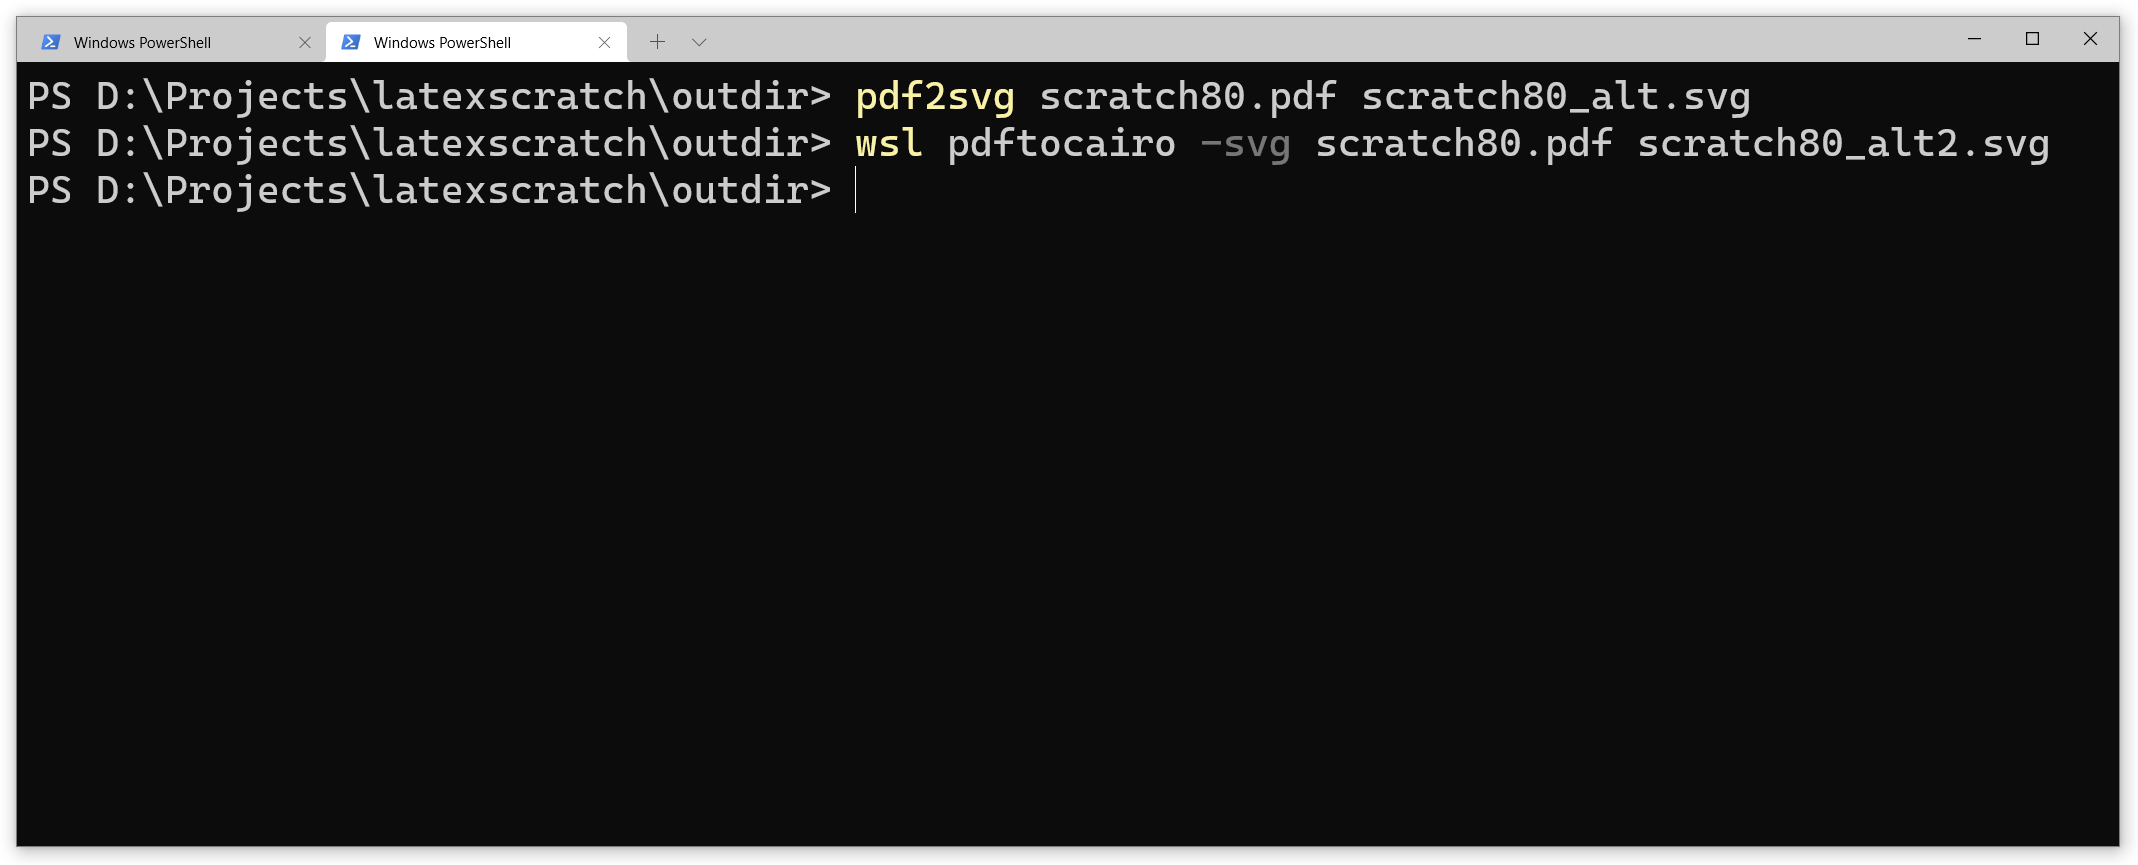
\includegraphics[width=\textwidth,height=0.8\textheight,keepaspectratio]{assets/convert_pdf_to_svg.png}
    \end{onlyenv}
    \begin{onlyenv}<+>
        \unless\ifishandout
        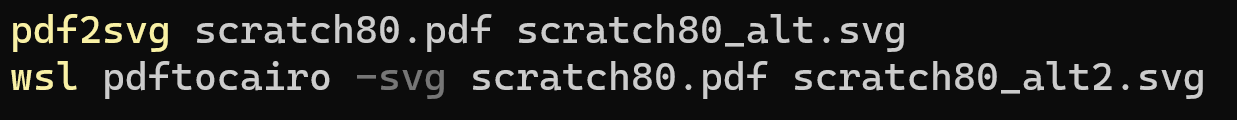
\includegraphics[width=\textwidth,height=0.8\textheight,keepaspectratio]{assets/convert_pdf_to_svg-small.png}
        \fi
    \end{onlyenv}

    Converteren van pdf naar svg met \hll|pdf2svg| of met package \hll|pdftocairo|. Voor laatste
    is Linux/Mac nodig of Windows Subsystem for Linux.
\end{frame}

\unless\ifishandout
\begin{frame}
    \begin{onlyenv}<+>
        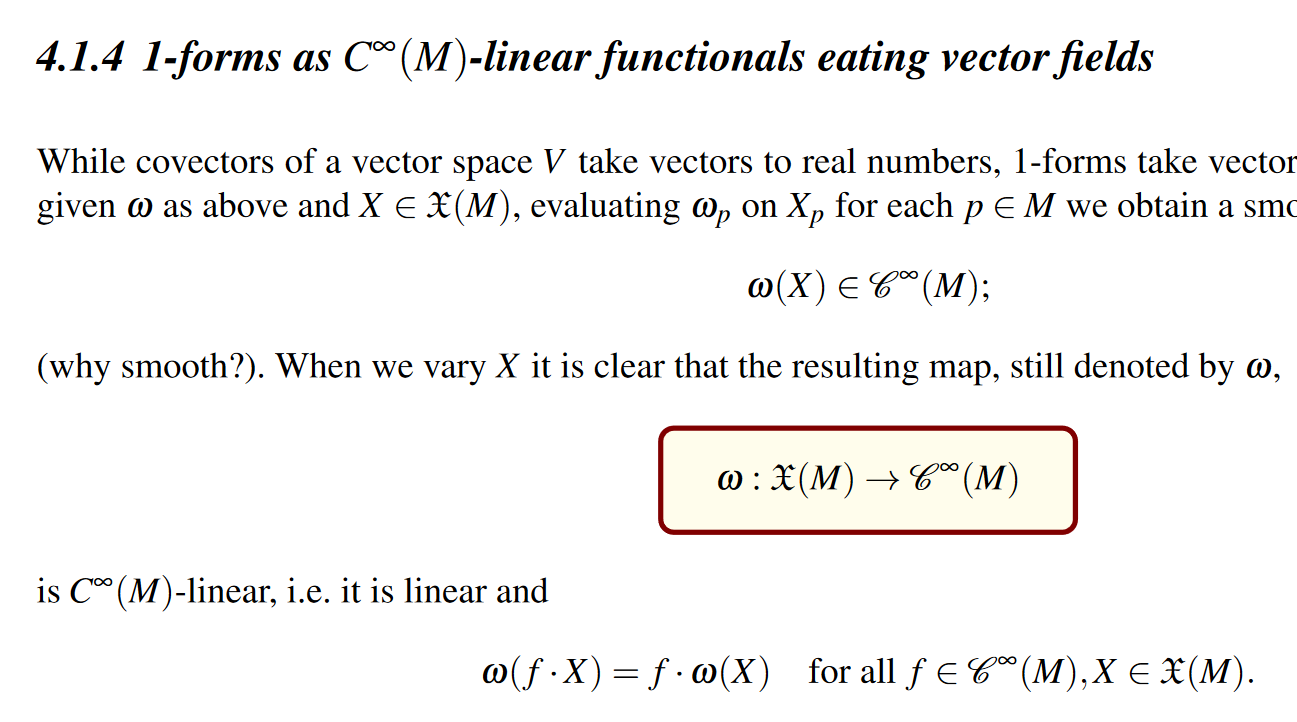
\includegraphics[width=\textwidth,height=0.8\textheight,keepaspectratio]{assets/pacman-before.png}
    \end{onlyenv}
    \begin{onlyenv}<+>
        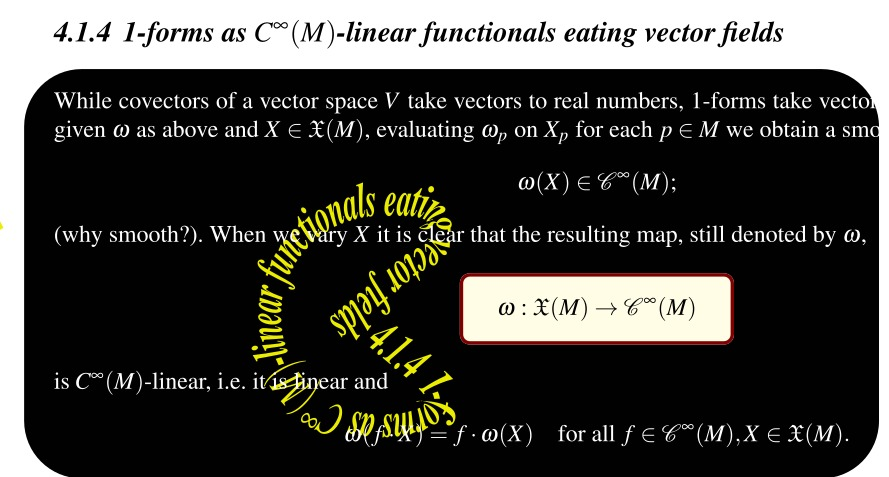
\includegraphics[width=\textwidth,height=0.8\textheight,keepaspectratio]{assets/pacman.jpg}
    \end{onlyenv}
    \begin{onlyenv}<+>
        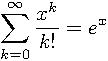
\includegraphics[width=\textwidth,height=0.8\textheight,keepaspectratio]{assets/document-standalone.pdf}
    \end{onlyenv}
    \begin{onlyenv}<+>
        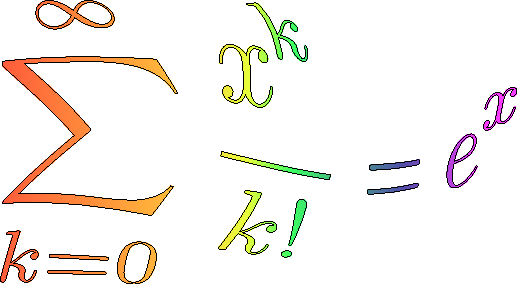
\includegraphics[width=\textwidth,height=0.8\textheight,keepaspectratio]{assets/formulaArt.pdf}
    \end{onlyenv}
\end{frame}
\fi
